% This is samplepaper.tex, a sample chapter demonstrating the
% LLNCS macro package for Springer Computer Science proceedings;
% Version 2.20 of 2017/10/04
%
\documentclass[runningheads]{llncs}
%
\usepackage{graphicx}
\usepackage{booktabs}
\usepackage{cite}
\usepackage{url}
\usepackage{multirow}
\usepackage{pgfplots}
\usepackage{tikz}
\usetikzlibrary{matrix,fit,shapes,calc,positioning,shadows,arrows,shapes,backgrounds,decorations.markings,fadings}
\usepackage{listings}
\usepackage[caption=false, font=footnotesize]{subfig}
%%%%%%%%%%%%% code listing
\renewcommand{\ttdefault}{pcr}
\lstset{
  basicstyle=\scriptsize\ttfamily,
  keywordstyle=\scriptsize\ttfamily\bfseries,
  language=C,             % choose the language of the code
  frame=single,              % adds a frame around the code
  aboveskip=0pt,
  belowskip=0pt,
  breaklines=true,           % sets automatic line breaking
  breakatwhitespace=false,   % sets if automatic breaks should only happen at
  showspaces=false,
  %numbersep=5pt,              % Abstand der Nummern zum Text
  %tabsize=2,                  % Groesse von Tabs
  %extendedchars=true,         %
  %breaklines=true,            % Zeilen werden Umgebrochen
  keywords=[2]{tcp, flag, threshold, track, count, seconds, classtype, sid}
}
\usepackage{balance}
\usepackage{wrapfig}
\usepackage{enumitem}
\usepackage{color, colortbl}
\definecolor{Gray}{gray}{0.9}

\newcommand{\tname}{\textsc{Syrius}} %% name of the technique
\newcommand{\ie}{i.e.}
\newcommand{\eg}{e.g.}
\newcommand{\aka}{a.k.a.}
\newcommand{\etal}{and colleagues}
\newcommand{\nids}{NIDS}
\newcommand{\metas}{Metasploit}
\newcommand{\suri}{Suricata}
\newcommand{\numrulessuri}{27.8K}
\newcommand{\percRulesWithContent}{93.5\%}
\newcommand{\numundetected}{\Fix{XX\%}}
\newcommand{\CodeIn}[1]{{\small{\texttt{#1}}}}
\newcommand{\MyComment}[1]{}

%% review
\newcommand{\Fix}[1]{{\textbf{[[}\color{magenta}#1}\textbf{]]}}
\newcommand{\Mar}[1]{{\textbf{[[Marcelo:~}\color{red}#1}\textbf{]]}}
\newcommand{\Luc}[1]{{\textbf{[[Lucas:~}\color{blue}#1}\textbf{]]}}
\newcommand{\Gui}[1]{{\textbf{[[Guilherme:~}\color{green}#1}\textbf{]]}}

\def\denseitems{
   \itemsep1pt plus1pt minus1pt
   \parsep0pt plus0pt
   \parskip0pt\topsep0pt}

%% numbers
\newcommand{\totoptions}{162}
\newcommand{\numproto}{11}
\newcommand{\totoptionsrelevant}{153}


% Used for displaying a sample figure. If possible, figure files should
% be included in EPS format.
%
% If you use the hyperref package, please uncomment the following line
% to display URLs in blue roman font according to Springer's eBook style:
% \renewcommand\UrlFont{\color{blue}\rmfamily}

\begin{document}
%
\title{Synthesis of Rules for Network Intrusion Detectors}
%
%\titlerunning{Abbreviated paper title}
% If the paper title is too long for the running head, you can set
% an abbreviated paper title here
%
\author{Lucas Alcantara\Comment{\inst{1}}\Comment{\orcidID{0000-1111-2222-3333}} \and
Guilherme Padilha\Comment{\inst{1}}\Comment{\orcidID{1111-2222-3333-4444}} \and
Marcelo d'Amorim\Comment{\orcidID{0000-0002-1323-8769}}}
%
\authorrunning{Alcantara et al.}
% First names are abbreviated in the running head.
% If there are more than two authors, 'et al.' is used.
%
\institute{Federal University of Pernambuco (UFPE), Recife, Brazil\\
\email{\{lama,ghps,damorim\}@cin.ufpe.br}}
%
\maketitle              % typeset the header of the contribution
%
\begin{abstract}
Network Intrusion Detection Systems (\nids{}) are a popular mechanism
used by system administrators to defend against network attacks. These
systems monitor the network traffic and flag suspicious network
behavior. Signature-based \nids\ do that by checking the network
traffic against a pre-defined set of rules, which can become obsolete
as attackers learn new strategies to circumvent existing defenses.
This paper proposes \tname{}\footnote{Abbreviation of \textbf{Sy}nthesis of
  Su\textbf{ri}cata R\textbf{u}le\textbf{s}.}, a technique that automatically
synthesizes \nids\ rules from positive and negative examples (\ie{},
malicious and benign traffic). \tname{} formulates synthesis as an
optimization problem whose candidate solutions are rules that
maximizes the captured the positive traffic and minimizes the captured
negative traffic. \tname{} bootstraps the search with candidate
solutions that use data from the payload of the malicious message and
produces optimal rule candidates on output. We evaluated \tname{} on a
diverse set of attacks. Results indicate that \Fix{...}

%% optimizes the
%% candidate solution to capture the positive example and, and then
%% optimizes the candidate solution to avoid capturing the negative
%% traffic. 


\keywords{NIDS, synthesis, search}
\end{abstract}
%
%
%
\section{Introduction}

Network Intrusion Detection Systems (\nids{}) are software systems
that monitor the network traffic for malicious behavior and act
accordingly by blocking messages or alerting humans about suspicious
events~\cite{Mitchell:2014:SID:2597757.2542049}. \nids{} are typically
placed behind a firewall, vetting the traffic that the firewall did
not block. Various open-source (\eg{}, Snort~\cite{snort} and
Suricata~\cite{suricata}) and commercial NIDS implementations (\eg{},
SolarWinds~\cite{solarwinds} and IBM QRadar~\cite{qradar}) exist
today. These systems are very popular in industry to secure local
computer networks given the amount of potential malicious traffic that
exist on the Internet.

\sloppy \nids{} are typically categorized in two
groups~\cite{kumar2007survey}: rule-based and anomaly-based \nids. A
rule-based intrusion detector\footnote{\aka\ signature-based intrusion
  detector.} checks if the network traffic matches a fixed set of
rules. Figure~\ref{fig:synflood-example} shows an example rule of
Suricata~\cite{suricata}, a popular open-source \nids{}. This rule
prescribes a method to capture a denial-of-service
attack~\cite{understanding-dos} to a server by matching specific
conditions about the network traffic. Relevant properties about the
traffic of interest appear in bold (see
Section~\ref{sec:suri-metas-coverage}). Rule-based \nids{} focus on
known attacks whereas anomaly-based \nids{} focus on unknown attacks
that could be observed by first learning the regular traffic and then
acting
properly~\cite{kumar2007survey,Mitchell:2014:SID:2597757.2542049,cordy-etal-issta19}. These
two kinds of intrusion detection mechanisms are
complementary. Rule-based NIDS could miss attacks (as rulesets can
become outdated) whereas anomaly-based NIDS can raise false alarms (as
detection algorithms are approximate).

Rule-based NIDS are restricted to a fixed set of rules defined by the
network system administrator. Manually writing these rules is tedious,
error-prone, but important as attackers constantly create new
strategies to circumvent existing rules. IT-security companies
capitalize on this phenomena and put rulesets on the market for
sale~\cite{proofpoint-etpro,snort-rule-subscriptions}.  Despite this
fundamental issue, rule-based systems are tremendously popular in
industry today. Anomaly-based NIDS are not restricted to a fixed set
of rules. They learn usage behavior from positive traffic and, based
on that, alert uncommon behavior~\cite{7579764}. Unfortunately,
anomaly-based NIDS are fundamentally imprecise. To sum up, rule-based
NIDS are precise but incomplete whereas anomaly-based NIDS are (more)
complete but imprecise.

%% This paper focuses on the
%% problem of discovering new rules by using anomaly-based NIDS.

This paper proposes \tname{}, a technique that uses machine
intelligence to automatically synthesize rules for rule-based
\nids. Our general goal is to harden the protection of NIDS by
improving the creation process of rules. One scenario of application
of \tname{} is one where an anomaly-based NIDS identifies abnormal
traffic and signals that traffic to \tname{} to create and distribute
the rules.

%% Note that anomaly-based NIDS are evolving pretty quick with the
%% advances in machine learning, but rule-based NIDS are still extremely
%% popular.  \tname{} could also leverage existing databases of malicious
%% traffic to synthesize rules.  Regardless of how the negative traffic
%% is produced (out of scope of this paper), those rules can be
%% distributed to rule databases for free.
%%  The
%% core motivation is that 1) attackers are productive in creating new
%% ways to circumvent existing protections and 2) manual creation of
%% rules is tedious and time-consuming.  

\tname{} synthesizes rules from positive and negative examples, \ie{},
malicious and benign traffic.

\Fix{summarize how the technique works}

\Fix{summarize results}

This paper makes the following contributions.

\section{Background}

This paper focuses on signature-based \nids. Although we focused on
the Suricata \nids, the principles we used are general to any other
signature-based \nids~(\eg{}, Snort~\cite{snort}).

\subsection{Suricata Rules}
\label{sec:example-suricata-rules}

Figure~\ref{fig:synflood-example} shows an example rule of
Suricata~\cite{suricata}, a popular open-source \nids{} maintained by
the Open Information Security Foundation (OISF)~\cite{oisf}. A
Suricata rule is divided in three parts---action, header, and rule
options~\cite{suri-rule-format}. The action part appears as the first
word in the rule description. An action denotes the task that needs to
be executed if the rule pattern is satisfied. In this example, a
message will be sent to system administrators if the rule pattern is
satisfied. The header comes after the action in the rule
description. It restricts the information flow covered by the
rule. For this rule, the header is \CodeIn{tcp \$HOME\_NET any ->
  \$EXTERNAL\_NET any}. It instructs Suricata to inspect \CodeIn{tcp}
traffic flowing from any port in the home network to any other address
outside the home network. The variables \CodeIn{\$HOME\_NET} and
\CodeIn{\$EXTERNAL\_NET} are configurable. The rule options come after
the header. It is a semi-colon-separated sequence of key-value
pairs. Options serve to 1) document the analyzed traffic (\eg{},
``msg'', ``classtype'', and ``sid'') and to 2) describe
characteristics of the attack (\eg, ``flags'', ``threshold'', and
``content''). \tname{} produces options of the second kind, which are
\emph{relevant} to capturing the attack.

Suricata supports a total of \totoptions\ distinct options covering
\numproto\ distinct protocols. A total of 9 of these options are for
documentation.
\begin{wrapfigure}[15]{r}{0.5\textwidth}
  \centering
  \vspace{-5ex}
  \scalebox{0.7}{
    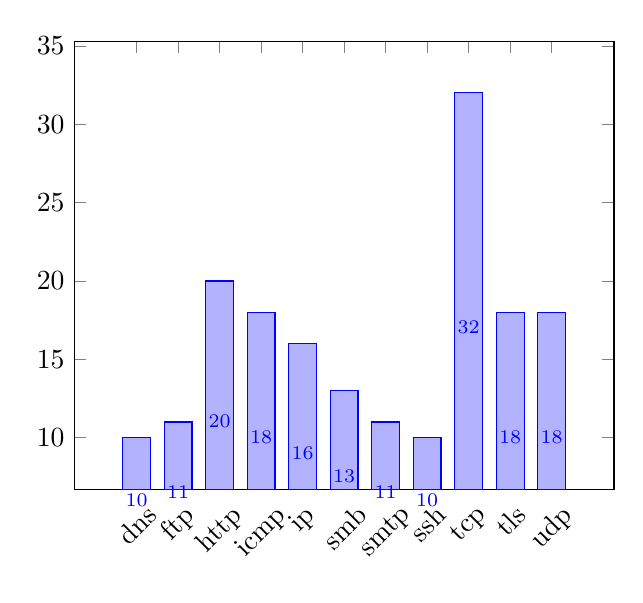
\begin{tikzpicture}
      \begin{axis}[
          ybar stacked,
          enlargelimits=0.15,
          legend style={at={(0.5,-0.15)},
            anchor=north,legend columns=-1},
          %          ylabel={\#rules},
          symbolic x coords={dns, ftp, http, icmp, ip, smb, smtp, ssh,
          tcp, tls, udp},
          xtick=data,
          xticklabel style={rotate=45},          
          nodes near coords,
          every node near coord/.append style={font=\scriptsize},        
          nodes near coords align={vertical},
        ]
        \addplot coordinates {(dns,10) (ftp,11) (http,20) (icmp,18)(ip,16) (smb,13) (smtp,11) (ssh, 10) (tcp, 32) (tls,18) (udp, 18)};
%        \legend{relevant, irrelevant}
      \end{axis}
    \end{tikzpicture}
  }
  \vspace{-1ex}
  \caption{\label{fig:distribution-rules-protocol}Number of relevant
    options per protocol supported by Suricata.}
\end{wrapfigure}
\Comment{For instance, the purpose of rule option \CodeIn{msg} is to print on
the output an informative message indicating what kind of intrusion
has been observed.} Figure~\ref{fig:distribution-rules-protocol} shows
the distributions of these options per protocol. The sum of
the number of protocol options is higher than \totoptions\ as some
options is shared across different protocols.

Table~\ref{table:rules} shows a sample of the options of
Suricata. Column ``\#'' shows the option number, column ``Name'' shows
the name of the option, column ``\#~Params'' shows the number of
additional parameters associated with a given option, and column
``Description'' presents a short description of the option purpose. We
found that the option \CodeIn{content} is particularly prevalent in
rules from public databases (see
Figure~\ref{fig:distribution-contents}). This option takes a sequence
of bytes as argument (\eg{}, \CodeIn{content:''SELECT ''}) and checks
if that sequence is present in the payload of the message. Detailed
description of the Suricata rules can be found
elsewhere~\cite{suri-rule-format}.

\begin{table}[h]
  \caption{\label{table:rules}Example options of Suricata.}  
  \centering
  \begin{tabular}{p{0.35cm}ll}
    \toprule
    \multicolumn{1}{c}{\#} & \multicolumn{1}{c}{Name} &  \multicolumn{1}{c}{Description}\\
    \midrule     
    1 & dsize & matches on the size of the packet payload\\
    2 & itype &  matches on a specific ICMP type\\
    3 & icode & matches on a specific ICMP code\\
    4 & icmp\_seq  & checks a ICMP sequence number\\
    5 & icmp\_id & matches on specific ICMP id-values\\
    6 & window & checks the size of the TCP window\\
    7 & flags & matches on TCP flags\\
    8 & fragbits & checks if the fragmentation or reserved bits are set in the IP header\\
    9 & threshold & controls the rule’s alert frequency\\
    10 & content & checks if argument is present on the payload\\
    \bottomrule
  \end{tabular}
\end{table}

\subsection{Rules and Packets}
\label{sec:rules-and-packets}

\Fix{Illustrate how information is extracted from packets}


\section{Illustrative Examples}
\label{sec:suri-metas-coverage}


This section briefly presents examples of attacks and rules that are
synthesized with \tname{} to capture those attacks.


\subsection{Denial-of-Service}

The SYN Flood attack is a denial-of-service attack that exploits a vulnerability in the TCP/IP handshake
to establish a TCP connection~\cite{cloudfare-synflood}. The handshake
works as follows in normal circumstances. First, a client sends a SYN
packet to the server, requesting a connection. Second, the server
responds with a SYN-ACK packet to the client. Third, the client
responds with an ACK message and the connection is established. Aware
of the protocol, an attacker sends multiple SYN packets to different
ports of a server, often using fake IP addresses. Then, after the
server responds with a SYN-ACK packet, the client keeps sending other
SYN packets to avoid the connection to time out. Without proper
protection, the server accepts these malicious requests and eventually
legitimate requests cannot be satisfied due to resource exhaustion.

\begin{figure}[h!]
  \lstinputlisting[language=C,numbers=none,keywords={flags,threshold}]{synflood.suricata}
  \caption{Suricata rule for SYN Flood Attacks.}
  \label{fig:synflood-example}
\end{figure}


Figure~\ref{fig:synflood-example} shows a Suricata rule that captures
this attack. This rule was obtained from the \Fix{...what source...}
The relevant options in the rule appear in bold---the option
\CodeIn{flags: S,12}, identifies a SYN packet in a TCP packet and the
option \CodeIn{threshold: type both, track by\_dst, count 5000,
  seconds 5} indicates that a high volume of such packets should be
requested in a short period of time.

%% Explain how \tname\ behaves on this attack



In the following, we illustrate how \tname{} proceeds for obtaining
the rule for the SYN Flood attack. The main challenge in synthesizing
rules is to discover the set of options that enables the \nids\ to
capture the malicious traffic, but ignore the benign traffic.  The
other parts of the rule (\ie{}, the action and the header) are either
inferred or left constant. \tname{} sets the action header to
\CodeIn{alert} and sets the header to \CodeIn{<proto> any any -> any
  any}, indicating that it infers the target protocol and uses the
most general flow description possible, \ie{}, it instructs the
\nids\ to analyze the traffic flowing from/to any address and port.
We understand that this is domain-specific information and conjecture
that the system administrator would know how to modify the constant
parts.

\tname{} proceeds as follows to synthesize rules for the SYN Flood
attack. First, it analyzes the positive traffic and extracts options
expressed in that traffic. For this example, it finds the following
set of options:

\Fix{atualize isto para o valor correto, por favor. $\rightarrow$}
\begin{figure}[h]
  \vspace{-3ex}
  \lstinputlisting[language=C,numbers=none,frame=none,keywords={flags,threshold}]{synflood.suricata.synth}
%  \caption{Suricata rule for SYN Flood Attacks.}
  %  \label{fig:synflood-example-synt}
  \vspace{-3ex}  
\end{figure}

Note that a rule that uses this set of options would capture the
positive traffic as these options originated from the positive
traffic. Unfortunately, such rule would be overspecified. It would
unlikely capture different manifestations of the same
attack. Informally, the rule includes ``too many'' characteristics of
the malicious traffic used to define it. To address this overfitting
issue, \tname{} minimizes the rule preserving the invariant that
plausible rules should only capture the positive traffic. \tname{}
potentially finds several minimal rules. The list below shows the
options for the five shortest rules it produces for this attack.

\Fix{...elaborate...}

\subsection{Active Reconnaissance}

Active reconnaissance is a method used by malicious individuals to
gather information about vulnerabilities from a computing system. The
most common approach is to ``scan'' open ports to discover
vulnerabilities. Active reconnaissance is a preliminary step towards
an attack that actually exploits the system. A Ping Scan is a very
common type of port scan based on the ICMP
protocol. \Fix{...explain this attack...}

\Fix{...explain how \tname\ works on it...}


\subsection{\Fix{...some other with contents...}}
\label{sec:content-example}

\Fix{...elaborate...}


%% \begin{table}[h]
%%   \caption{\label{table:rules}Rule evolution}  
%%   \centering
%%   \begin{tabular}{lllll}
%%     \toprule
%%     \multicolumn{1}{c}{Iteration} & \multicolumn{1}{c}{Rule} \\
%%     \midrule     
%%     0 & (ack:0; seq:0; window:0; flags:F;)\\
%%     5 & (window:0; flags:F;)\\
%%     68 & (window:64; flags:F;)\\
%%     73 & (window:64; flags:S,12;)\\
%%     94 & (window:64; flags:S,12; threshold: type both, track by\_dst, count 20, seconds 1;)\\
%%     \bottomrule
%%   \end{tabular}
%% \end{table}

\section{Technique}

\tname{} is a technique that uses positive and negative examples to
synthesize signature-based NIDS rules, such as those from Snort and
Suricata. The goal of \tname\ is to create a rule that \emph{only}
captures the positive traffic, \ie{}, the malicious sequence of
messages.

\begin{figure*}[t]
\centering
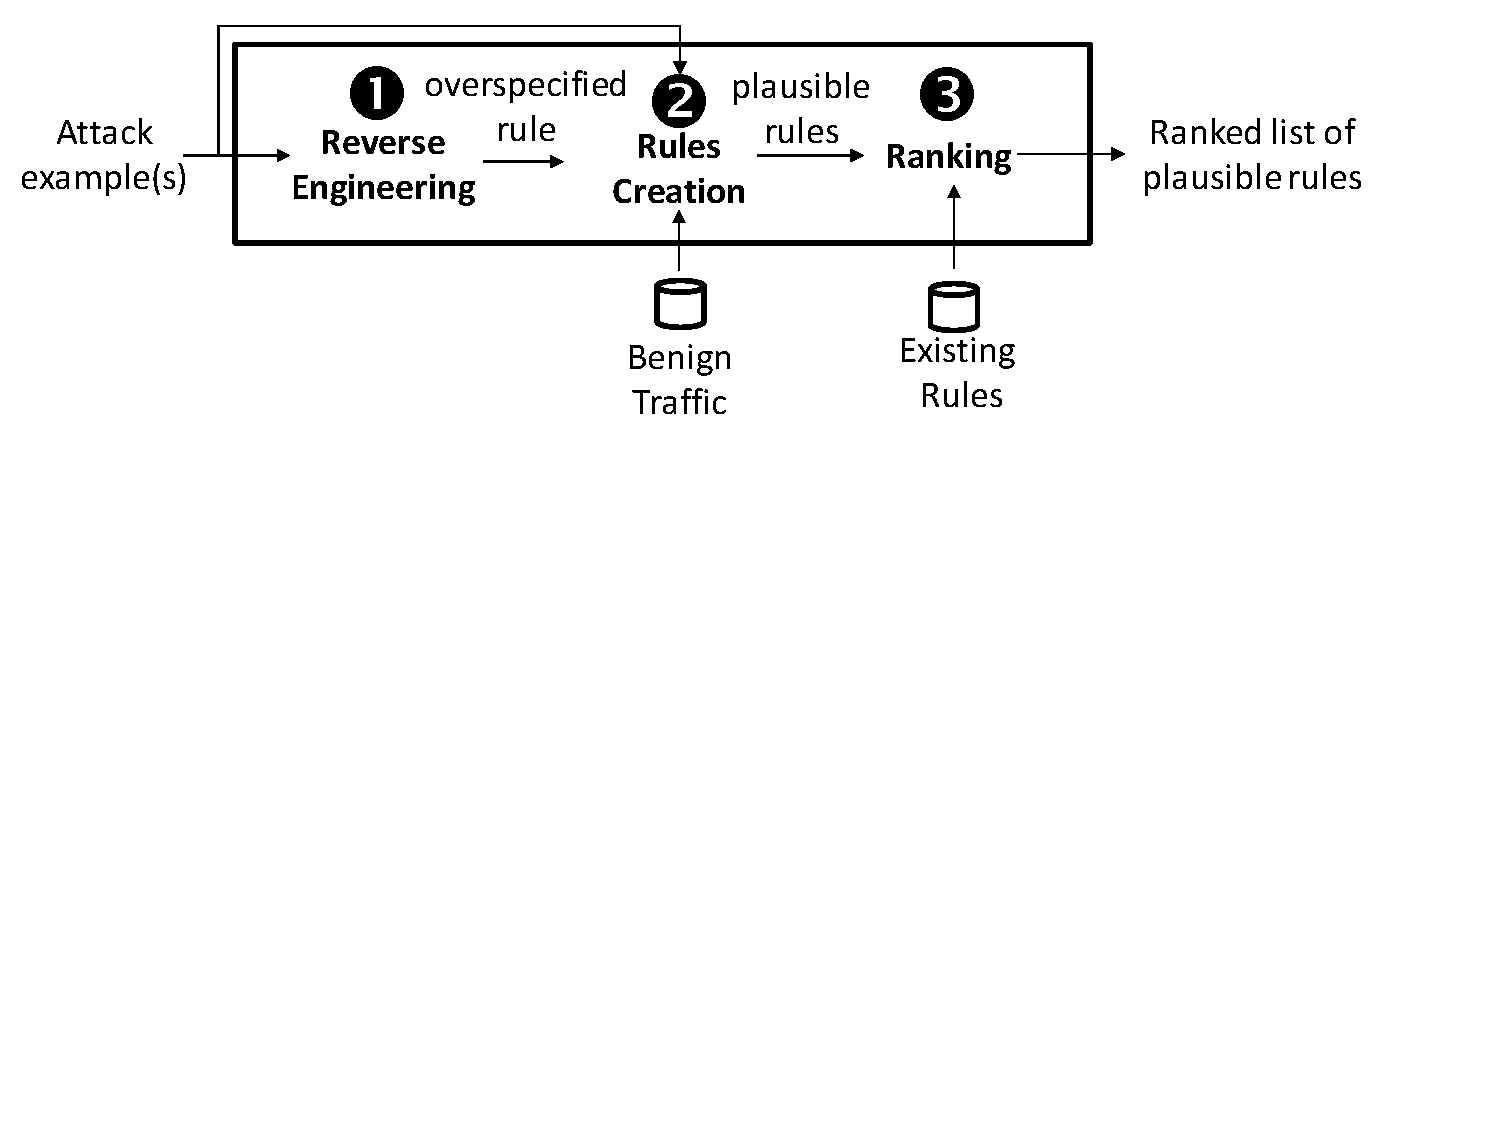
\includegraphics[trim=0 300 350 0,clip,width=0.95\textwidth]{figs/nids-workflow}
\caption{\tname\ workflow.}
\label{fig:overview}
\end{figure*}

\vspace{1ex}
\noindent\textbf{Overview.}~ The input of the technique is the
positive traffic whereas the output is a list of minimized rules
capturing only the positive, malicious,
traffic. Figure~\ref{fig:overview} shows the workflow of \tname{} as a
pipeline of two components, which appear numbered in the figure.
\tname{} synthesizes rules in two steps. First, it produces a
potentially overspecified rule that captures the malicious traffic
provided on input. In this step, \tname\ finds options by
\emph{reverse engineering} the positive traffic. It extracts tokens
from the malicious message and uses them to define the initial
rule. We say that this rule overfits the problem as it satisfies the
success criterion of only capturing the positive traffic, however it
is unlikely that it will be able to generalize to other attacks,
\ie{}, attacks of the same kind, but with different data. The reason
is that many options added to the rule are unimportant for
discriminating the attack. In the second step, \tname{} uses negative
examples to \emph{minimize} the rule, discarding unnecessary
options. Note that any subset of the original set of options captures
the positive traffic. The minimization step uses a population-based
gradient descent-like search to generate minimal solutions.





%% The goal of the first
%% component is to produce a rule that captures the negative traffic.
%% First, it initializes the rule with random values. Only options
%% associated with the used protocol are included in the rule
%% representation. Then, \tname\ optimizes the rule options until
%% \suri\ is able to capture the attack associated with the negative
%% traffic.  \tname\ unsuccessfully terminates at this point if it cannot
%% capture the attack. The second component takes as input the rule
%% produced by the first component and tries to minimize that rule. Note
%% that any subset of options would capture the negative traffic---as all
%% options in the rule need to be satisfied for the negative traffic to
%% be captured---but it can also capture positive traffic. This component
%% systematically discards options from the rule encoding until no
%% positive traffic is captured.



\subsection{Step 1: Reverse Engineering}
\pgfplotsset{width=6cm,compat=1.8}
\pgfplotsset{every tick label/.append style={font=\tiny}}

\begin{wrapfigure}[14]{r}{0.56\textwidth}
  \centering
  \vspace{-8ex}
  \scalebox{1.2}{  
    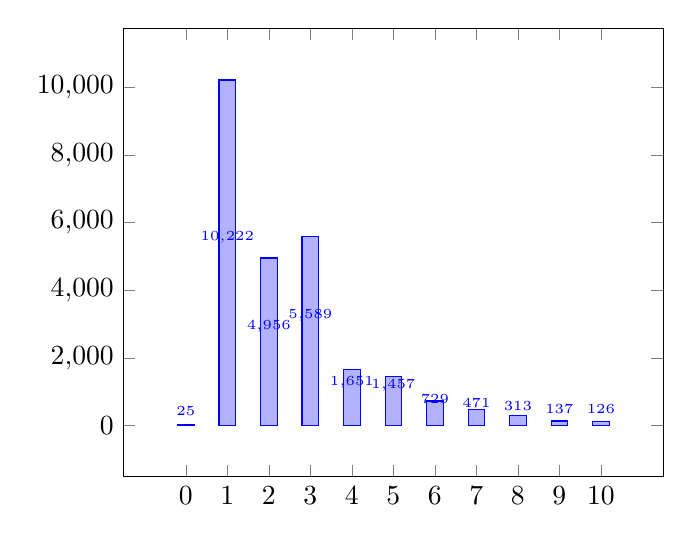
\begin{tikzpicture}
      \begin{axis}[
          bar width=6pt,
          scaled ticks=false,
          tick label style={/pgf/number format/fixed},
          ybar stacked,
          enlargelimits=0.15,
          legend style={at={(0.5,-0.15)},
            anchor=north,legend columns=-1},
          symbolic x coords={0, 1, 2, 3, 4, 5, 6, 7, 8, 9, 10},
          xtick=data,
          nodes near coords,
          every node near coord/.append style={font=\tiny},
          nodes near coords align={vertical},
        ]
        \addplot coordinates {(0,25) (1,10222) (2,4956) (3,5589)
          (4,1651) (5,1457) (6, 729) (7, 471) (8, 313) (9, 137) (10, 126)};
      \end{axis}
    \end{tikzpicture}
  }
  \caption{\label{fig:distribution-contents}Histogram of number of
    \CodeIn{content} options per rule (up to 10).}
\end{wrapfigure}
The goal of the first step is to extract options from the positive
traffic. For that, \tname{} parses the protocol message, looking for
fields in the message associated with options (see
Section~\ref{sec:rules-and-packets}). For example, fields
\Fix{...and...}  can be used to determine the option
\Fix{zzz}. Unfortunately, inferring options at the field granularity
level is insufficient to capture \CodeIn{content} options (see
Section~\ref{sec:example-suricata-rules}), which refer to parts of the
payload of the message and cannot be directly extracted directly from
the fields. Handling this case is critically important as most rules
contain \CodeIn{content}
options. Figure~\ref{fig:distribution-contents} shows the histogram of
number of these options per rule (up to 10) for the Suricata public
rule database \Fix{cite}. Rules without \CodeIn{content} options is an
exception and half of the rules contain at least two \CodeIn{content}
options.  To find the values associated with these options, \tname{}
splits the payload of the malicious message in tokens using natural
language delimiters, such as $\backslash$t, $\backslash$n,
$\backslash$r, and spaces. The rationale for this decision is that we
observed, by inspecting existing rules, that \CodeIn{content} options
typically refer to sequence of characters in the payload of messages
separated by these delimiters. This tokenization step can generate
dozens of options. For the example from
Section~\ref{sec:content-example}, \tname{} produces a total of
\Fix{xx} content options.

\subsection{Step 2: Rule Minimization}

\Fix{--------------------------- estou aqui}

The rule reported by the first step satisfies the criterion to only
capture positive traffic, however it is ``too'' specific---it is
unable to capture different manifestations of the same attack as the
rule would unlikely match exactly the options we found for the input
message. Some options added to the rule during the first step are
irrelevant for determining the attack and should be removed.

The goal of this step is to create a \emph{minimal} rule that captures
\emph{only} the positive malicious traffic. A rule is minimal if
discarding any option results in capturing negative (\ie{}, benign)
traffic. Recall that the previous maximization step produces a rule
that captures the positive traffic and all options are satisifed by
the positive traffic. Consequently, any subset of these options also
captures the positive traffic. The minimization procedure we propose
in this step builds on that observation. It iteratively discards
options from the candidate rule until no other options can be
removed. The procedure uses negative traffic to guide the
search. Public databases of negative traffic with \Fix{thousands} of
messages exist \Fix{cite cite} and can be used to increase the
accuracy of the minimization.

\subsection{Limitations}

\Fix{...}

\section{Evaluation}

%% \renewcommand{\labelitemi}{}
%% \setitemize[0]{leftmargin=20pt,itemindent=-20pt}
%% \begin{itemize}
%% \end{itemize}

%% \renewcommand{\labelitemi}{}
%% \setitemize[0]{leftmargin=0pt,itemindent=0pt}
%% \begin{itemize}
%%   \item{\textbf{RQ1.}~How precise is \tname?}
%%   \item{\textbf{RQ2.}~How efficient is \tname?}
%% \end{itemize}

This section reports precision and efficiency of \tname.


\subsection{Objects of Analysis}

We evaluated \tname{} on a set of attacks covering each of the four
protocols supported by Suricata and attacks with different
characteristics. Table~\ref{table:attacks} shows the attacks we
analyzed and the rule of Suricata that captures the attack. Column
``Name'' shows the name of the attack, column ``\#'' indicates whether
single or multiple messages are required to manifest the attack,
column ``Protocol'' shows the protocol name, column ``Description''
summarizes the effect of the attack, if successfull, and column
``Golden Rule'' shows the relevant parts in the options section of the
Suricata rule that captures the attack.

\begin{table*}[t!]
  \caption{\label{table:attacks}Characterization of attacks analyzed
    and Golden Rule of Suricata (reference) to capture it.\Mar{please,
  show me the Golden Rule, \ie{} the part that is relevant of each rule (for
  capturing the negative traffic precisely)}}  
  \centering
  \begin{tabular}{lllll}
    \toprule
    \multicolumn{1}{c}{Name} & \multicolumn{1}{c}{\#} & \multicolumn{1}{c}{Protocol} & \multicolumn{1}{c}{Description} & \multicolumn{1}{c}{Golden Rule} \\
    \midrule     
    Ping Scan & single & ICMP & Discovers active hosts in a network &  dsize:0; itype:8; \\
    Black Nurse & multiple & ICMP & Denial of Service & itype:3; icode:3; detection\_filter:track by\_dst, count 250, seconds 1;\\
    Ping Flood  & multiple & ICMP & Denial of Service & itype:8; icode:0; detection\_filter:track by\_src, count 30, seconds 1;\\  
    Port Scan TCP & single & TCP & Discovers open ports in a host & flags: A; ack: 0;dsize: 0; \\
    SYN Flood & multiple & TCP & Denial of Service & flags: S,12; threshold: type both, track by\_dst, count 5000, seconds 5;\\
    UDP Flood & multiple & UDP & Denial of Service & fragbits:M; threshold: type both, track by\_dst, count 5000, seconds 5; \\
    \bottomrule
  \end{tabular}
\end{table*}

\subsection{Setup}

Note from Figure~\ref{fig:overview} that the negative traffic is an
input to the technique. The positive (non malicious) traffic, in
contrast, is not. \tname{} uses public databases storing different
kinds of positive traffic for all protocols covered by Suricata. We
used two datasets of positive traffic. The Bigflows.pcap dataset is
part of the TcpReplay~\cite{tcpreplay} open source project. This
dataset includes real network traffic on a busy private network access
point to the Internet. According to the TcpReplay web site ``This
capture is much larger and has a smaller average packet size than the
previous capture (smallFlows.pcap). It also has many more flows and
different applications.''. In addition to the Bigflows.pcap dataset,
we also used datasets of normal traffic made available by Stratosphere
Lab~\cite{stratosphere-normal}.

%% \Gui{We are using the bigflows.pcap provided by tcpreplay on http://tcpreplay.appneta.com/wiki/captures.html "This is a capture of real network traffic on a busy private network’s access point to the Internet"
%%  }

\Luc{entrada: utilizamos a ferramenta hping3 para executar o ataque em um alvo arbitrario dentro da rede (n ha necessidade de haver um alvo real para executar o hping3) e capturamos o trafego gerado com o wireshark. o comando utilizado foi:\\*
\texttt{\# hping3 -d 80 -w 64 -S -p 80 --flood --rand-source 192.138.1.115} \\*
que envia pacotes de 80 bytes (-d 80), com a flag SYN habilitada (-S), tamanho de janela de 64 bytes (-w 64), direcionados a porta 80 (-p 80). A flag --flood indica q o hping3 vai enviar os pacotes o mais rápido possível. a flag --rand-source indica que cada pacote vai ter um ip de origem aleatorio. 192.138.1.115 é o alvo.\\*
O trafego armazenado contem 40 mil pacotes SYN, enviados no intervalo de 1 segundo,  pegamos uma amostra de 20 desses pacotes para representar o flood e servir como entrada.\\*
O wireshark armazena os pacotes no formato pcap, utilizamos a ferramenta tcpreplay para reproduzir o trafego com o comando:\\*
\texttt{\# tcpreplay --pps 200 --intf1=wlp2s0 Datasets/syn-flood-sample.pcap}\\*
Nesse caso, estamos enviando os pacotes armazenados em \texttt{Datasets/syn-flood-sample.pcap} a uma taxa de 200 pacotes por segundo (\texttt{-pps 200}) utilizando a interface wlp2s0 (\texttt{--intf1 wlp2s0})\\* 
Há diferenças entre os pacotes na opção ack.\\* 
Por que 20? Apenas para gerar a regra mais rapidamente, poderia ser qualquer valor maior ou menor. No final, o parâmetro \texttt{count} da opção \texttt{threshold} vai ser alterado pelo adm da rede.\\*
Intervalo de reprodução: 0.005 segundo

}

\Fix{any other detail we should consider?}

\subsection{Precision}

\Fix{...}

\subsection{Efficiency}

\Fix{...}

\section{Threats to Validity}

External Validity. \Fix{elaborate ...how popular are Suricata/Metasploit?}

\section{Related Work}

\Fix{...}
%
% ---- Bibliography ----
%
% BibTeX users should specify bibliography style 'splncs04'.
% References will then be sorted and formatted in the correct style.
%
\bibliographystyle{splncs04}
\bibliography{references}
%

\end{document}
